% This is LLNCS.DEM the demonstration file of
% the LaTeX macro package from Springer-Verlag
% for Lecture Notes in Computer Science,
% version 2.4 for LaTeX2e as of 16. April 2010
%
\documentclass[citenumber]{elsarticle}
\newtheorem{proposition}{Proposition}
\newtheorem{definition}{Definition}
\newtheorem{proof}{Proof}
\newtheorem{corollary}{Corollary}

\usepackage{hyperref}				% enlaces en el pdf
\hypersetup{colorlinks=true,        % colores en vez de cajas en los enlaces
			linkcolor=blue,         % color of internal links (change box color with linkbordercolor)
    		citecolor=blue,         % color of links to bibliography
    		filecolor=blue,         % color of file links
    		urlcolor=blue}          % color of external links	    

\usepackage{algorithm,algpseudocode}
\usepackage{multicol}
\usepackage{graphicx}           	% para manejar imagenes
\usepackage[utf8]{inputenc}
\usepackage{pstricks,pst-node,pst-tree} % Para la taxonomía
\usepackage{stackengine}				% Para listar los articulos en el nodo de la taxonomía
%\usepackage[table]{xcolor}			% Colores en el cronograma
%\usepackage{algorithm}				% Para el seudocódigo
%\usepackage{setspace}				% Para el seudocódigo
%\usepackage{amsmath}					% Para el seudocódigo
%\usepackage[noend]{algpseudocode}	% Para el seudocódigo
%\usepackage{multicol}				% Para el seudocódigo
%\usepackage{algorithmic}

\usepackage{tikz}
\usetikzlibrary{arrows}

\tikzset{
  treenode/.style = {align=center, inner sep=0pt, text centered,
    font=\sffamily},
%  circ/.style = {treenode, circle, white, font=\sffamily\bfseries, draw=black,
%    fill=black, text width=1.5em},% arbre rouge noir, noeud noir
  circ/.style = {treenode, circle, black, draw=black, 
    text width=1.5em, very thick},% arbre rouge noir, noeud rouge
  disc/.style = {treenode, circle, draw=gray,fill=gray,
    minimum width=1.5em, very thick}% arbre rouge noir, nil
}

\renewcommand{\algorithmicrequire}{\textbf{Input:}}
\renewcommand{\algorithmicensure}{\textbf{Output:}}

%-------------------------------------------------------------------------
% Configuring Taxonomy
%-------------------------------------------------------------------------
\setstackEOL{\\}
\def\psedge{\ncangles[angleA=-90,angleB=90]}
\psset{levelsep=20mm,treesep=1cm,nodesep=3pt, arrows=->}
\def\PSBL#1{\small\pspicture(7,0.5)\psTextFrame[shadow,
  fillstyle=solid,linecolor=blue,framearc=0.3](0,0)(7,0.5){%
    \shortstack{#1}}\endpspicture}
\def\PSBS#1{\pspicture(2.2,.5)\psTextFrame[shadow,
  fillstyle=solid,linecolor=blue,framearc=0.3](0,0)(2.2,0.5){%
    \shortstack{#1}}\endpspicture}

%-------------------------------------------------------------------------
% Referencias a una palabra
%-------------------------------------------------------------------------
\newcommand{\setword}[2]{%
  \phantomsection
  #1\def\@currentlabel{\unexpanded{#1}}\label{#2}%
}



\begin{document}
%\mainmatter              % start of the contributions
%
\title{A parallel implementation of the fast--BR algorithm for reduct computation}

	\author[inaoe,uc]{Vad\'{\i}mir~Rodr\'{\i}guez-Diez\corref{cor1}}
	\ead{vladimir.rodriguez@inaoep.mx}
	\address[inaoe]{Computer Science Department\\
					Instituto Nacional de Astrof\'{\i}sica, \'{O}ptica y Electr\'{o}nica\\
					Luis Enrique Erro \# 1, Santa Mar\'{\i}a Tonantzintla, Puebla, 72840, M\'{e}xico} 
	\address[uc]{Electrical Engineering Department\\
				 Universidad de Camag\"{u}ey\\
				 Circv. Nte. km 5$\frac{1}{2}$, Camag\"{u}ey, Cuba}

%
\begin{abstract}
%
	Rough set theory is a relatively new mathematical theory to deal with imperfect knowledge, in particular with vague concepts. One of the key concepts within rough set theory is the concept of reduct. A reduct is a reduced set of attributes for the description of an dataset without changing its discernibility relations. The main limitation of rough set reducts is that computing the complete set of reducts of a dataset has exponential complexity regarding the number of attributes. Several attempts have been made to speed up reduct computation but most of these solutions looks for a subset of reducts.  This research proposal aims to develop a parallel implementation of the fast--BR algorithm, which is one of the fastest algorithms reported in the literature for reduct computation.
%
\end{abstract}
%
	\maketitle
%
\section{Introduction}
%
	Rough set theory (RST), proposed by Z. Pawlak in 1982 \cite{Pawlak81}, is a relatively new mathematical theory to deal with imperfect knowledge, in particular with vague concepts. Into RST, datasets are tables of objects (rows) described by a set of attributes (columns). When data is collected or recorded, every single aspect (attribute) of the object under study is considered to have a complete representation and to ensure that no potentially useful information is lost. As a result, datasets are usually characterized by a large number of attributes,  degrading the performance of machine learning tools \cite{Parthalain08}. One of the main concepts in RST is the notion of reduct, which is a minimal subset of attributes preserving the discernibility capacity of the whole set of attributes \cite{Pawlak91}. However, the main restriction of RST is that computing all reducts of a dataset has exponential complexity \cite{Skowron92}. Therefore, the development of fast algorithms for reduct computation is an active research line.
  
	Several attempts to speed up the reduct computation have been reported. Many of these algorithms are based on some heuristics. Another explored way to speed up reduct computation is parallelization \cite{Strakowski08}. There are also interesting alternatives such as the use of a parallel version of genetic algorithms \cite{Wroblewski98} and the transformation of the reduct computation problem to the well known SAT problem \cite{Jensen14}.
	
	RST reducts have been related to Typical Testors (TT) from the logical combinatorial approach to pattern recognition \cite{Chikalov2013}. Testor Theory was originally created by Cheguis and Yablonskii \cite{Cheguis55} as a tool for analysis of problems connected with control and diagnosis of faults in circuits. However, Testor Theory has been extended in order to be used for feature selection as shown in \cite{Dmitriev1966,Martinez01,Ruiz08}. Algorithms for typical testor computation can be applied to reduct computation due to the similarity between these two concepts \cite{Lazo15}. 
	
	The complete set of reducts of a dataset is useful for solving some practical problems and real--world applications. In \cite{Xu2013} a multi-objective cost-sensitive attribute reduction was developed. First, they compute all reducts of a dataset. Then, they separately calculate the cost, in terms of time and money, of every reduct. Finally, the worst reducts are dismissed, leaving a Pareto optimal solution set. From this smaller set of reducts, a user can easily select an optimum subset. On the other hand, in \cite{Mukamakuza2014} three new algorithms for dynamic reduct computation were developed. The first step in the three algorithms is finding of all reducts. Then, the complete set of reducts is filtered in order to obtain an optimum subset, from which dynamic reducts are computed. They showed that this procedure improves the performance of dynamic reduct computation algorithms. From Testor Theory \cite{Torres2014}, the informational weight, computed through typical testors (reducts), was used to identify risk factors on transfusion related to acute lung injury; and to establish an assessment for each attribute. In \cite{Torres2014}, the informational weight for an attribute is computed as the percentage of times the attribute appears in the whole set of typical testors. 
	  
	Recently, the relation between reduct computation and the minimum vertex cover problem in graph theory was exposed \cite{chen2015}. Given that both of these problems can be translated into the calculation of prime implicants of a Boolean function, they applied algorithms designed for reduct computation in the solution of the minimum vertex cover problem. This unification opens a new spectrum of real-world applications for fast reduct computation algorithms. They stood that the vertex cover problem has been used in applications such as crew scheduling~\cite{Sherali1984}, VLSI design \cite{Bhattacharyya2000}, nurse rostering \cite{Caprara1998} and industrial machine assignments~\cite{Woodyatt1993}. The connection with the problem of computing the prime implicants of a Boolean function makes fast algorithms for computing all reducts relevant in other applications. For instance, in \cite{Li2015} a new technique for mining frequent patterns from the minimal disjunctive normal form was presented.
	
	In this research proposal, we ...
%

\section{Related Work}\label{relatedWork}
  In this section, we will first discuss heuristic algorithms for reduct computation. Some of these algorithms are capable of finding several reducts and others are intended to obtain a single \textit{shortest} reduct. Afterwards, we will give an overview of those algorithms reported for computing all reducts. Finally, we will make a review of parallel accelerations of algorithms for reduct computation reported in the literature.    
%	
\subsection{FPGA accelerations}
%
  
%	
\subsection{Parallel accelerations}
%
	
%
\section{Research Proposal}  
%        
	\begin{table}[htb]
		\caption{Simplified Binary Discernibility Matrix.} \label{tab:SBDM}
		\centering
	 	\begin{tabular}{cccccc}
	 		$x_0$ & $x_1$ & $x_2$ & $x_3$ & $x_4$ & $x_5$ \\
	 		\hline
			1 & 1 & 0 & 0 & 0 & 0 \\
			0 & 0 & 0 & 1 & 0 & 0 \\
			0 & 0 & 1 & 0 & 0 & 0 \\
			0 & 0 & 0 & 0 & 0 & 1 \\
			1 & 0 & 0 & 0 & 1 & 0
	 	\end{tabular}             
 	\end{table}
 
 \begin{table}[htb]
 		\caption{Candidates evaluated by fast--BR on the \textit{SBDM} shown in Table~\ref{tab:SBDM}.} \label{tab:cand}
 		\footnotesize
 		\centering
 		\setlength{\tabcolsep}{3pt}
 	 	\begin{tabular}{cl|cl|cl|cl|cl}
 	 		n & candidate & n & candidate & n & candidate & n & candidate & n & candidate \\
 	 		\hline
			1 & ${x_0}$     & 6  & ${x_0,x_5}$         & 11 & ${x_1}$     & 16 & ${x_1,x_2,x_3}$     & 21 & ${x_1,x_2,x_3,x_4,x_5}$  \\
			2 & ${x_0,x_1}$ & 7  & ${x_0,x_2,x_3}$     & 12 & ${x_1,x_2}$ & 17 & ${x_1,x_2,x_4}$     &   \\
			3 & ${x_0,x_2}$ & 8  & ${x_0,x_2,x_5}$     & 13 & ${x_1,x_3}$ & 18 & ${x_1,x_2,x_5}$     &   \\
			4 & ${x_0,x_3}$ & 9  & ${x_0,x_2,x_3,x_5}$ & 14 & ${x_1,x_4}$ & 19 & ${x_1,x_2,x_3,x_4}$ &   \\
			5 & ${x_0,x_4}$ & 10 & ${x_0,x_3,x_5}$     & 15 & ${x_1,x_5}$ & 20 & ${x_1,x_2,x_3,x_5}$ &       
 	 	\end{tabular}             
  	\end{table}	
 	
 	
	% First Tree
	\begin{figure}[htb]
		\center
		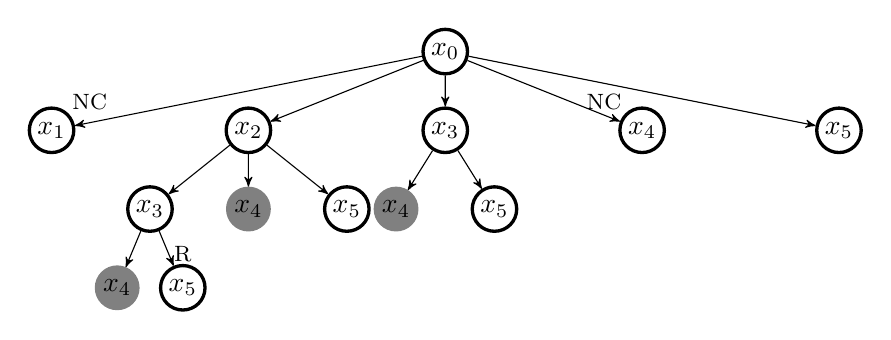
\begin{tikzpicture}[->,>=stealth',level/.style={sibling distance = 2.5cm/#1,
		  level distance = 1cm}] 
		\node [circ] {$x_0$}
		    child{ node [circ] {$x_1$}   
		    node[above right=0.4em] {\footnotesize{NC}}
		    }
		    child{ node [circ] {$x_2$} 
		        child{ node [circ] {$x_3$} 
					child{ node [disc] {$x_4$}}
					child{ node [circ] {$x_5$}
						    node[above=0.6em] {\footnotesize{R}}
					}
		        }
		        child{ node [disc] {$x_4$}}
		        child{ node [circ] {$x_5$}}
			}
			child{ node [circ] {$x_3$}
				child{ node [disc] {$x_4$}}
				child{ node [circ] {$x_5$}}
			}
			child{ node [circ] {$x_4$}
			node[above left=0.4em] {\footnotesize{NC}}
			}
			child{ node [circ] {$x_5$}}
		; 
		\end{tikzpicture}
		\caption{Evaluation of supersets of $x_0$.}
		\label{fig:tree1}
	\end{figure}
	
	% Second Tree
	\begin{figure}[htb]
		\center
		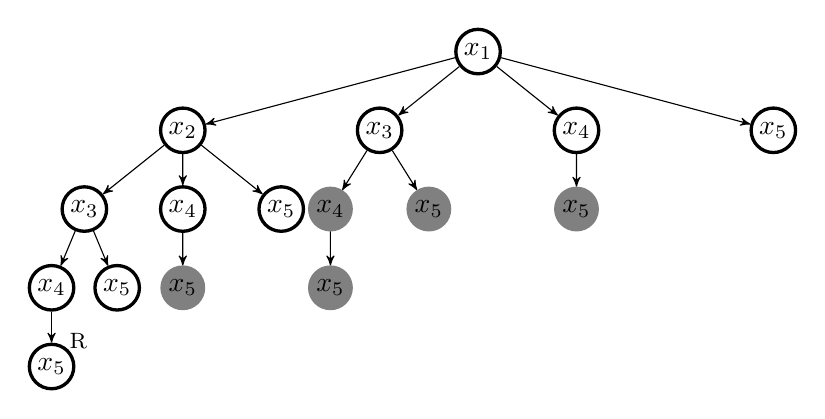
\begin{tikzpicture}[->,>=stealth',level/.style={sibling distance = 2.5cm/#1,
		  level distance = 1cm}] 
		\node [circ] {$x_1$}
		    child{ node [circ] {$x_2$} 
		        child{ node [circ] {$x_3$} 
					child{ node [circ] {$x_4$}
						child{ node [circ] {$x_5$}
							    node[above right=0.3em] {\footnotesize{R}}
						}
					}
					child{ node [circ] {$x_5$}}
		        }
		        child{ node [circ] {$x_4$}
		        	child{ node [disc] {$x_5$}}
		        }
		        child{ node [circ] {$x_5$}}
			}
			child{ node [circ] {$x_3$}
				child{ node [disc] {$x_4$}
					child{ node [disc] {$x_5$}}
				}
				child{ node [disc] {$x_5$}}
			}
			child{ node [circ] {$x_4$}
				child{ node [disc] {$x_5$}}
			}
			child{ node [circ] {$x_5$}}
		; 
		\end{tikzpicture}
		\caption{Evaluation of supersets of $x_1$.}
		\label{fig:tree2}
	\end{figure}
%
\section{Previous Research Work} \label{preliminary}
%

%
\section{Concluding Remarks}\label{conclusions}
%
   From our literature review, we highlight the following aspects. First, we found that algorithms for computing rough set reducts are mainly divided into three categories:
    \begin{itemize}
  	  \item Algorithms for computing a pseudo-optimal reduct according to a criterion (which is, most of the 
  	  		time, the cardinality of the obtained reduct).
  	  \item Algorithms for computing one shortest reduct.
  	  \item Algorithms for computing all reducts.
    \end{itemize}
    The most proliferative research area in Rough Set Theory is the development of algorithms for computing a 
    pseudo-optimal reduct. 
    
    We found two algorithms for finding all reducts \cite{Starzyk00,WangP07} and two algorithms for finding shortest reducts \cite{Lin04,Jensen14}. These algorithms have several disadvantages since they do not work over the simplified discernibility matrix and use complex data representations. Notice that computing the simplified binary discernibility matrix from the original dataset has Quartic complexity regarding the number of objects (rows) in the dataset, while computing all reducts has exponential complexity regarding the number of attributes (columns). In most computationally expensive datasets, it is better to work over the simplified discernibility matrix. 
    
    Hardware accelerations of algorithms for computing reducts are focused on computing a single pseudo-optimal reduct \cite{Tiwari11,Tiwari12,Tiwari13,Grzes13,Kopczynski14,Tiwari14}. Since this problem is not an exponentially complexity task, we found these hardware platforms less useful.	
		    
    In the search for algorithms to overcome the exponential complexity of the problem of computing all reducts or
    shortest reducts, the last word has not been said. Two promising areas of research are the hardware acceleration of algorithms computing all reducts and the palletization of these algorithms.
  
% ---- Bibliography ----
%
\bibliographystyle{authordate1}
\bibliography{mybib}

\end{document}